\documentclass[a4paper, 11pt, titlepage]{article}
\usepackage[utf8]{inputenc}
\usepackage[english]{babel}
\usepackage[]{parskip}
\usepackage{graphicx}
\usepackage{xcolor}
\usepackage{paralist} % compactitem
\usepackage{csquotes}
\usepackage{wrapfig}
\usepackage{subfig}
\usepackage{csvsimple} % csv tables

% Title spacing
\usepackage{titlesec}
\titlespacing*{\section}{0pt}{0pt}{0pt}
\titlespacing*{\subsection}{0pt}{-5pt}{-5pt}
\titlespacing*{\subsubsection}{0pt}{0pt}{0pt}

% Read data from file
\usepackage{datatool}
\DTLsetseparator{ = }
\DTLloaddb[noheader, keys={key,value}]{knndata}{data/knn_acc}
\DTLloaddb[noheader, keys={key,value}]{neighborhooddata}{data/neighborhood_acc}
\DTLloaddb[noheader, keys={key,value}]{perceptrondata}{data/perceptron_err}

% Citations
\usepackage[
  style=ieee,
  citecounter,
  labelnumber,
  backend=biber,
  bibencoding=utf8,
  sorting=none
]{biblatex}
\addbibresource{references.bib}

% Code blocks
\usepackage{listings}
\definecolor{codegreen}{rgb}{0,0.6,0}
\definecolor{codegray}{rgb}{0.5,0.5,0.5}
\definecolor{codepurple}{rgb}{0.58,0,0.82}
\definecolor{backcolour}{rgb}{1.0,1.0,1.0}
\lstdefinestyle{mystyle}{
  backgroundcolor=\color{backcolour},
  commentstyle=\color{codegreen},
  keywordstyle=\color{magenta},
  numberstyle=\tiny\color{codegray},
  stringstyle=\color{codepurple},
  basicstyle=\ttfamily\tiny,
  breakatwhitespace=false,
  breaklines=true,
  captionpos=b,
  keepspaces=false,
  numbersep=5pt,
  showspaces=false,
  showstringspaces=false,
  showtabs=false,
  tabsize=2
}
\lstset{style=mystyle}

% Custom commands
% Referencing
\newcommand{\figRef}[1]{Fig. \ref{#1}}
\newcommand{\tabRef}[1]{Tab. \ref{#1}}
\newcommand{\eqRef}[1]{(\ref{#1})}
% Reading data from files
\newcommand{\knnData}[1]{\DTLfetch{knndata}{key}{#1}{value}}
\newcommand{\neighborhoodData}[1]{\DTLfetch{neighborhooddata}{key}{#1}{value}}
\newcommand{\perceptronData}[1]{\DTLfetch{perceptrondata}{key}{#1}{value}}

\title{EECE6036 - Homework 2}
\author{Wayne Stegner}
\date{\today}

\begin{document}
  \maketitle
  \section{Problem 1}
  \subsection{Problem Summary}
  \par In this problem, two spatial-neighborhood classifiers are investigated
  to classify people as either ``Stressed'' or ``Not Stressed'' based on
  previous and current income.
  The k-Nearest Neighbors (KNN) classifies based on the $k$ nearest points,
  while the Neighborhood algorithm classifies based on the points within a
  radius $R$.
  In this implementation of the Neighborhood algorithm, ties in the
  distribution of classes in the neighborhood will default to ``Not Stressed''
  The goal of this problem is to find optimal $k$ and $R$ for these algorithms
  when applied to the given dataset.
  \subsection{Results}
  \par The balanced accuracy metrics for KNN and Neighborhood classifiers are
  shown in \figRef{fig:knn_bal_acc} and \figRef{fig:neighborhood_bal_acc}
  respectively.
  The values of $k$ were from 1 to 99 to get a better idea of the scalability
  of $k$, using only the odd numbers to avoid ties in the class distribution of
  the neighbors.
  The values of $R$ were from 0 to 10 incrementing by 0.2 to observe the
  behavior of $R$ over a large range.
  The optimal value for $k$ is \knnData{bestk} with a balanced accuracy of
  \knnData{acc}\%, and the optimal value for $R$ is \neighborhoodData{bestr}
  with a balanced accuracy of \neighborhoodData{acc}\%.
  \begin{figure}[htb]
    \center
    \vspace{-20pt}
    \subfloat[]{
      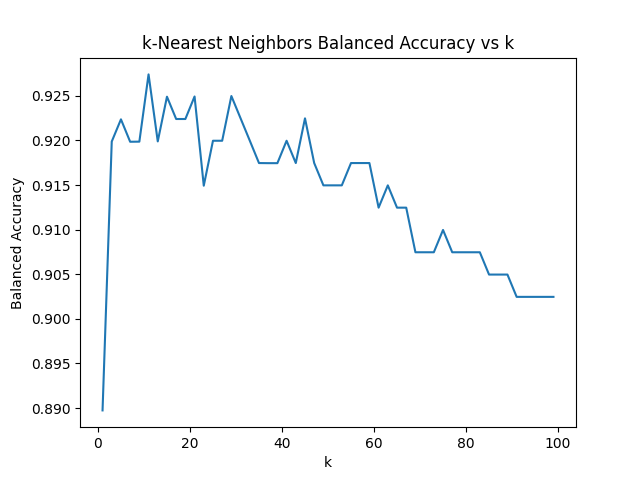
\includegraphics[width=0.47\textwidth]{images/knn_bal_acc.png}
      \label{fig:knn_bal_acc}
    }
    \subfloat[]{
      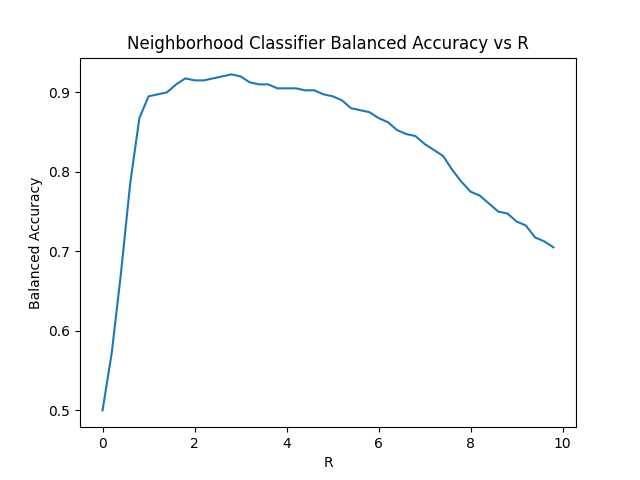
\includegraphics[width=0.47\textwidth]{images/neighborhood_bal_acc.png}
      \label{fig:neighborhood_bal_acc}
    }
    \vspace{-5pt}
    \caption{Balanced accuracy for KNN (a) and Neighborhood Classifier (b).}
    \vspace{-15pt}
    \label{fig:neighbor_bal_acc}
  \end{figure}
  \subsection{Discussion}
  \par KNN is slightly more accurate than the Neighborhood method.
  However, KNN has the advantage that it will always have a neighborhood with
  a consistent size and no ties (if $k$ is odd).
  This dataset contains some sparse regions which may yield few or no neighbors
  for some points, but increasing $R$ to accommodate for those regions will
  cause large neighborhoods in the dense regions to hold disproportionately
  many points.
  \subsection{Conclusion}
  The optimal $k$ value is \knnData{bestk} and the optimal $R$ value is
  \neighborhoodData{bestr}.
  Both algorithms classify this dataset to over 92\%.
  \pagebreak

  \section{Problem 2}
  \subsection{Problem Summary}
  In this problem, the same dataset is classified using a single perceptron
  using a simple training algorithm.
  For this problem, the dataset was split into 80\% training and 20\% testing.
  The purpose of this problem is to try different learning rates, training
  epochs, and weight initialization strategies.
  \subsection{Results}
  The error (1 - balanced accuracy) for both training and testing after
  training for \perceptronData{epochs} at a learning rate of
  \perceptronData{learning_rate} is shown in \figRef{fig:perceptron_error}.
  The final training error is \perceptronData{train_err}, and the final testing
  error is \perceptronData{test_err}.
  Because this dataset is 2-dimensional, it was simple to choose a range of
  weights that would go across the dataset.
  \par To get the desired general position, the bias weight is initialized on a
  uniform distribution between -10 and -50, while the input weights are
  initialized on a uniform distribution between 2 and 5.
  The axis intercepts can be calculated as $\frac{-w_{bias}}{w_{input}}$, which
  will be between 5 and 25 with the selected ranges.
  This range will put the initial decision boundary close to the data.
  \par The learning rate and training epochs were found empirically.
  The learning rate was started out as 0.1, then adjusted down by a factor of
  10 until the error curve smoothed out and settled down.
  The number of epochs was set based on the learning rate to observe the error
  bottom out, or continue to oscillate for the higher learning rates.
  \begin{figure}[htb]
    \center
    \vspace{-10pt}
    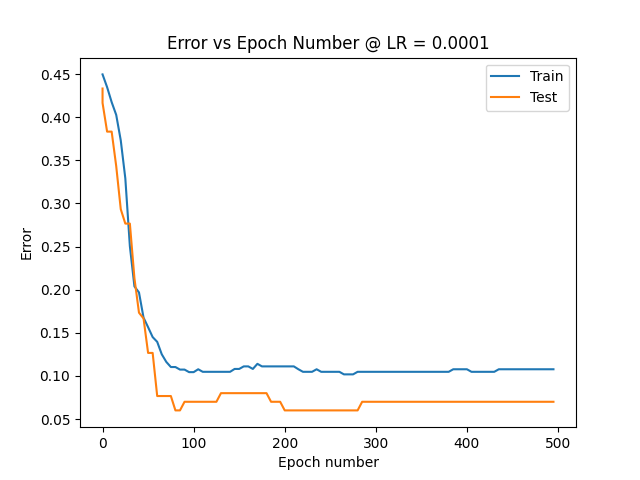
\includegraphics[width=0.47\textwidth]{images/perceptron_err.png}
    \vspace{-5pt}
    \caption{Training and testing error for a single perceptron.}
    \vspace{-15pt}
    \label{fig:perceptron_error}
  \end{figure}
  \subsection{Discussion}
  \par These results indicate that the perceptron is successfully training on
  the data, because the error decreases over time and stays low.
  Training appears to be finished around 100 epochs, but it is safer to train
  a bit longer (150 epochs) just in case the initial decision boundary is
  worse.
  \subsection{Conclusion}
  The perceptron should be trained with a learning rate of
  \perceptronData{learning_rate} for 150 epochs to ensure full training.
  \pagebreak

  \section{Problem 3}
  \subsection{Problem Summary}
  \par The purpose of this problem is to compare the performance of the three
  classifiers using the optimal parameters from Problems 1 and 2.
  This will be done over nine trials, in which each algorithm will classify a
  random 80\% train/20\% test partition of the dataset.
  For each trial, the perceptron has a random initialization of the weights as
  described in Problem 2.
  Performance metrics are measured for each trial, including balanced accuracy,
  precision, recall, and F1 score.
  \subsection{Results}
  \subsubsection{Performance on Individual Trials}
  \par The performance metrics for the individual trials of the KNN,
  Neighborhood, and perceptron classifiers are shown in \figRef{fig:knn_perf},
  \figRef{fig:neighborhood_perf}, and \figRef{fig:perceptron_perf}
  respectively.
  \begin{figure}[htb]
    \centering
    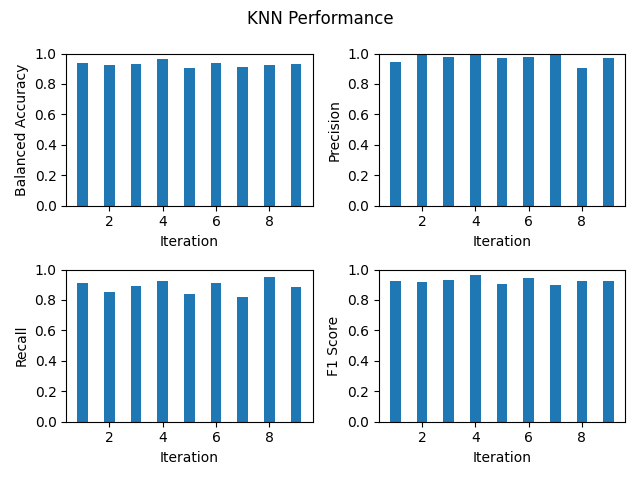
\includegraphics[width=0.5\textwidth]{images/knn_performance.png}
    \caption{Performance metrics for the KNN classifiers.}
    \label{fig:knn_perf}
  \end{figure}
  \begin{figure}[htb]
    \centering
    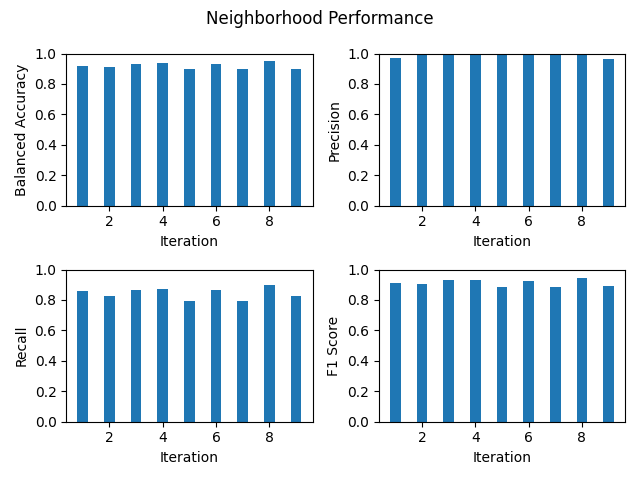
\includegraphics[width=0.5\textwidth]{images/neighborhood_performance.png}
    \caption{Performance metrics for the Neighborhood classifiers.}
    \label{fig:neighborhood_perf}
  \end{figure}
  \begin{figure}[htb]
    \centering
    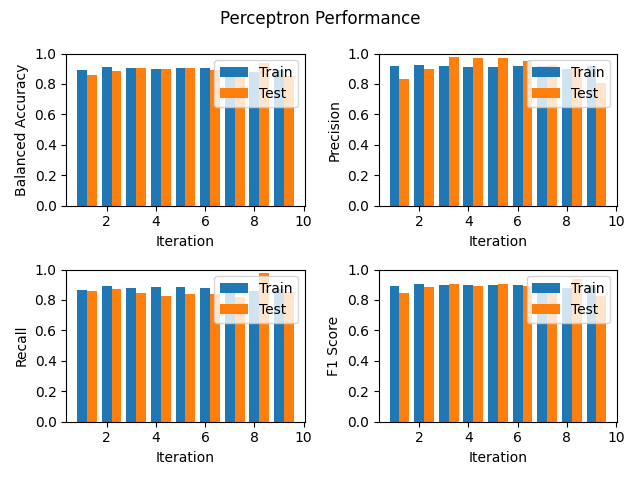
\includegraphics[width=0.5\textwidth]{images/perceptron_performance.png}
    \caption{Performance metrics for the perceptron classifiers.}
    \label{fig:perceptron_perf}
  \end{figure}
  \subsubsection{Average Performance}
  \par \tabRef{tab:avg_perf} shows the average and standard deviation
  performance metrics for the classifiers aggregated over all nine trials.
  \begin{table}[htb]
    \caption{Average performance of the classifiers.}
    \begin{center}
      \csvautotabular{data/avg_perf.csv}
    \end{center}
    \label{tab:avg_perf}
  \end{table}
  \subsubsection{Trial-Wise Training Error for the Perceptrons}
  \par The trial-wise training error for each of the nine perceptrons over the
  duration of training is shown in \figRef{fig:trial_err}.
  \begin{figure}[htb]
    \centering
    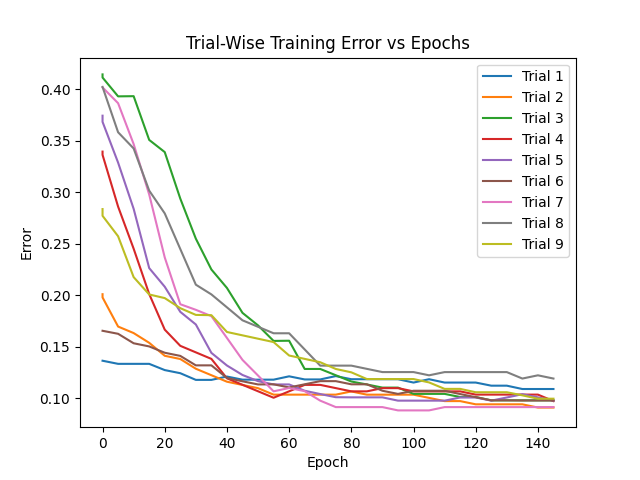
\includegraphics[width=0.5\textwidth]{images/trial_wise_error.png}
    \caption{Trial-wise training error of perceptrons over training duration}
    \label{fig:trial_err}
  \end{figure}
  \subsubsection{Mean Training Error for the Perceptron}
  \par The mean and standard deviation training error for each of the nine
  perceptrons over the duration of training is shown in \figRef{fig:mean_err}.
  \begin{figure}[htb]
    \centering
    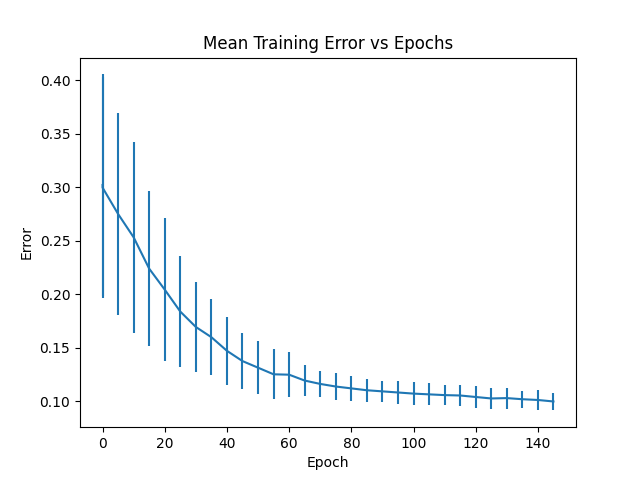
\includegraphics[width=0.5\textwidth]{images/mean_error.png}
    \caption{Mean training error of perceptrons over training duration.}
    \label{fig:mean_err}
  \end{figure}
  \subsubsection{Best KNN Decision Boundary}
  \par The decision boundary for the KNN classifier with the highest balanced
  accuracy is shown in \figRef{fig:knn_dec}.
  This boundary was calculated by sampling the input space with 100 divisions
  in both the N range (0 to 23) and the P range (0 to 14).
  \begin{figure}[htb]
    \centering
    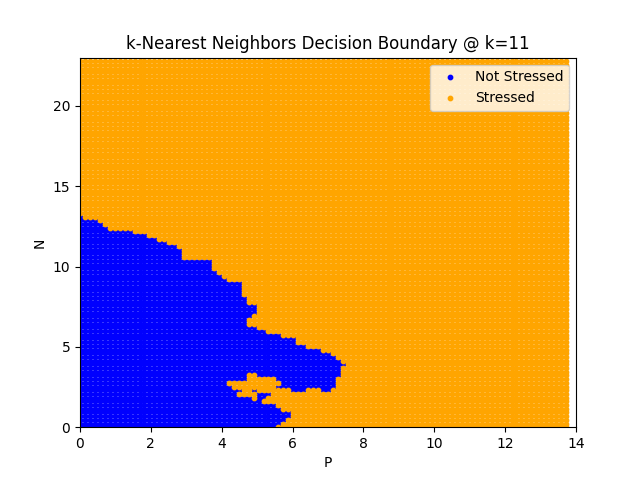
\includegraphics[width=0.5\textwidth]{images/knn_dec_bound.png}
    \caption{Decision boundary for the best KNN classifier.}
    \label{fig:knn_dec}
  \end{figure}
  \subsubsection{Best Neighborhood Classifier Decision Boundary}
  \par The decision boundary for the Neighborhood classifier with the highest
  balanced accuracy is shown in \figRef{fig:neighborhood_dec}.
  This boundary was calculated using the same method as the KNN.
  The blue regions in the upper left and right corners are an artifact of the
  tie resolution method, which is to default to a ``Not Stressed''
  classification.
  \begin{figure}[htb]
    \center
    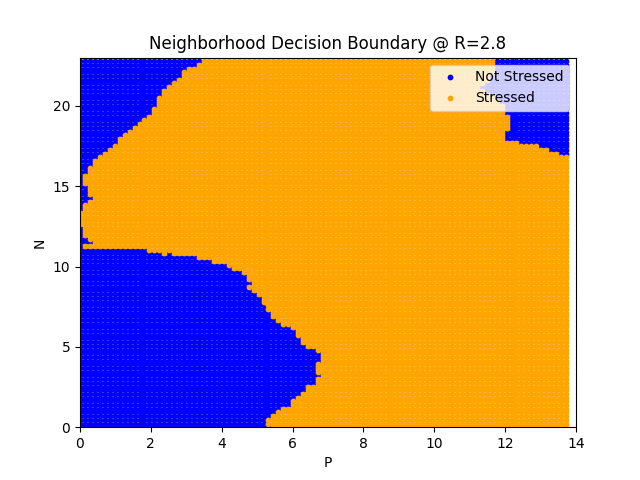
\includegraphics[width=0.5\textwidth]{images/neighborhood_dec_bound.png}
    \caption{Decision boundary for the best Neighborhood classifier.}
    \label{fig:neighborhood_dec}
  \end{figure}
  \subsubsection{Perceptron Decision Boundary}
  \par The decision boundary for the perceptron unit with the highest balanced
  accuracy is shown in \figRef{fig:perceptron_dec}.
  This boundary was calculated based on the weights of the trained unit.
  \begin{figure}[htb]
    \center
    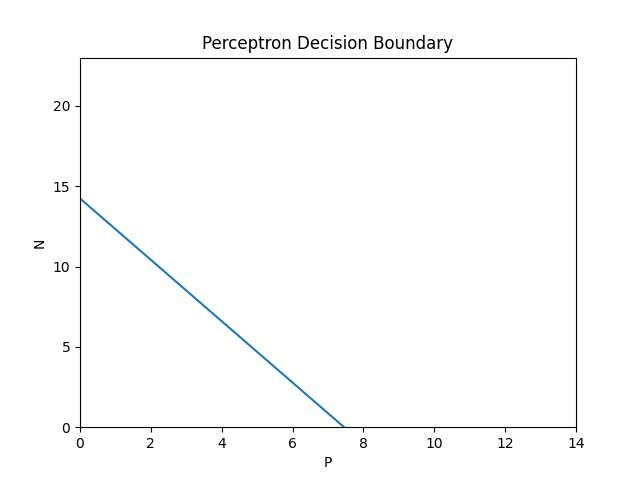
\includegraphics[width=0.5\textwidth]{images/perceptron_dec_bound.png}
    \caption{Decision boundary for the best perceptron unit.}
    \label{fig:perceptron_dec}
  \end{figure}
  \subsubsection{Analysis of Results}
  % Analyse suitability for this problem
  \par These algorithms all exhibit the ability to classify the given dataset,
  with each of them having balanced accuracies of near or just above 90\%
  averaged over all nine trials, shown in \tabRef{tab:avg_perf}.
  The standard deviations are all relatively low, indicating that all of the
  trials had similar ability to classify the testing set.
  Therefore, it is safe to say that all of the classification algorithms have
  the ability to classify this particular dataset.
  % Opinion of the pros and cons of each
  \par These algorithms each have pros and cons.
  The KNN classifier is advantageous in that it has the ability to generate a
  nonlinear decision boundary, as shown in \figRef{fig:knn_dec}.
  Additionally, it has the guarantee that each point will have enough neighbors
  to make a classification.
  On the negative side, the KNN decision boundary can over-fit.
  Additionally, because each point is guaranteed to have neighbors, these
  neighbors might be spatially distant for outliers, which may lead to a
  classification that does not make sense.
  \par The Neighborhood classifier, like the KNN classifier, has the ability to
  produce nonlinear decision boundaries, as shown in
  \figRef{fig:neighborhood_dec}.
  In contrast to the KNN, the Neighborhood classifier guarantees that all
  neighbors are spatially close.
  However, because neighbors are based on proximity, points with either equal
  distributions of classes in the neighbors or no neighbors at all may be
  misclassified.
  For this implementation, the default for those cases was a classification of
  ``Not Stressed,'' which causes all outliers to be in that class.
  With datasets with a mix of dense and sparse data points, it will be
  challenging to find a radius where all sparse points have neighbors, but the
  dense points do not have extraneous amounts of neighbors.
  \par The perceptron can only produce a linear decision boundary as shown in
  \figRef{fig:perceptron_dec}, which can be viewed as both a pro and a con.
  On the positive side, the linear decision boundary is simpler than the KNN
  and Neighborhood decision boundaries, and achieves comparable results.
  However, the negative side is that it will only work for linearly separable
  data.
  Another negative side is that it takes time to train the unit, while KNN and
  Neighborhood do not.
  However, the classification calculation by the perceptron is much simpler,
  because it only has to do a few multiplications and summations, rather than
  calculating Euclidean distance for every single reference point.
  % Recommendation for one with justification
  \par While each of the classifiers exhibit reasonably good performance, based
  on this study I will recommend the KNN for this particular dataset.
  The KNN outperforms the Neighborhood classifier in every metric presented in
  \tabRef{tab:avg_perf} except for precision, and the precision of the KNN was
  only about 2\% worse for the KNN.
  While the linear decision boundary of the perceptron allows for quick
  classification, the perceptron performed the worst in every metric.
  Additionally, this dataset is not strictly linearly separable, and there is
  significant overlap between the two classes that cannot be captured by a
  single perceptron.
  \subsection{Discussion}
  \par The KNN, Neighborhood, and perceptron classifiers all were able to
  classify this dataset.
  They each have pros and cons, but in the end the KNN is probably the best
  classifier for this dataset.
  That being said, the recommendation may change if more data is acquired which
  suggests that the KNN was merely over-fit to this dataset, and a linear
  decision boundary is more accurate.
  In that case, the perceptron would be better.
  \subsection{Conclusion}
  \par While all three algorithms were able to classify the dataset, the KNN is
  the most recommended classifier for this particular case.
  \pagebreak
  \appendix
  \section{Code}
  \subsection{\texttt{dataset.py}}
  \lstinputlisting[language=python]{"code/dataset.py"}
  \subsection{\texttt{classifier.py}}
  \lstinputlisting[language=python]{"code/classifier.py"}
  \subsection{\texttt{knn.py}}
  \lstinputlisting[language=python]{"code/knn.py"}
  \subsection{\texttt{neighborhood.py}}
  \lstinputlisting[language=python]{"code/neighborhood.py"}
  \subsection{\texttt{perceptron.py}}
  \lstinputlisting[language=python]{"code/perceptron.py"}
  \subsection{\texttt{problem\_3.py}}
  \lstinputlisting[language=python]{"code/problem_3.py"}
\end{document}
